\documentclass[twoside]{article}

% We add packages, macros here:
%!TEX root =  lec-template.tex
\usepackage{lmodern}
\usepackage[english]{babel}
\usepackage{latexsym}
\usepackage{amsmath}
\usepackage{mathrsfs}
\usepackage{amssymb}
\usepackage{mathtools}
\usepackage[inline,shortlabels]{enumitem} % we prefer enumitem because of its margin adjustment caps
\usepackage{bm}
\usepackage{datetime}
\usepackage[table,xcdraw]{xcolor}
\usepackage{accents}
\usepackage{tikz}
\usepackage{listings}
\usepackage{mdframed}
\usepackage{pgfplots}
\usepackage{pgfplotstable}
\usepackage[boxed]{algorithm}
\usepackage{algpseudocode}
\usepackage{dsfont}
\usepackage{color}
\usepackage{colortbl}
\usepackage{pifont}
\usepackage[bf,font=small,singlelinecheck=off]{caption}
\usepackage{microtype} % improved spacing between words for easier reading
\usepackage{float}
\usepackage{xfrac} % sfrac
\usepackage{xspace}

\linespread{1.1}


\usepackage[textsize=tiny]{todonotes}
\makeatletter
\renewcommand{\todo}[2][]{\@todo[#1]{#2}}
\makeatother

\setlength{\marginparwidth}{10ex}
\newcommand{\todoc}[2][]{\todo[size=\scriptsize,color=blue!20!white,#1]{Csaba: #2}}
\newcommand{\todoj}[2][]{\todo[size=\scriptsize,color=red!20!white,#1]{Jincheng: #2}}

\usepackage{hyperref}
\hypersetup{
    unicode=false,          % non-Latin characters in Acrobat�s bookmarks
    pdftoolbar=true,        % show Acrobat�s toolbar?
    pdfmenubar=true,        % show Acrobat�s menu?
    pdffitwindow=false,     % window fit to page when opened
    pdfstartview={FitH},    % fits the width of the page to the window
    pdftitle={},    % title
    pdfauthor={},     % author
    pdfsubject={Theory, Machine Learning, Lectures},   % subject of the document
    pdfcreator={},   % creator of the document
    pdfproducer={}, % producer of the document
    pdfkeywords={theory} {machine learning} {lecture notes} {CMPUT 654} {Fall 2023}, % list of keywords
    pdfnewwindow=true,      % links in new window
    colorlinks=true,       % false: boxed links; true: colored links
    linkcolor=blue,          % color of internal links (change box color with linkbordercolor)
    citecolor=blue,        % color of links to bibliography
    filecolor=magenta,      % color of file links
    urlcolor=cyan           % color of external links
}
\usepackage{amsthm}
\usepackage{times}
\usepackage{natbib}
\usepackage{nicefrac}
\usepackage{wrapfig}
\usepackage[capitalize]{cleveref}
\usepackage[nottoc,numbib]{tocbibind}

%\usepackage[bmargin=0.75in]{geometry}
\usepackage[margin=1.1in]{geometry}
\usepackage[normalem]{ulem}


%%%%%%%%%%%%%%%%%%%%%%%%%%%%%%%%
% HYPHENATION
%%%%%%%%%%%%%%%%%%%%%%%%%%%%%%%%

\pretolerance=5000
\tolerance=9000
\emergencystretch=0pt
\righthyphenmin=4
\lefthyphenmin=4


\bibliographystyle{plainnat}

\newcommand{\E}{\mathbb{E}}
\newcommand{\EE}[1]{\E[#1]}
\newcommand{\PP}{\mathbb{P}}
\newcommand{\Prob}[1]{\mathbb{P}(#1)}
\newcommand{\one}[1]{\mathbb{I}\{#1\}}
\newcommand{\Supp}{\operatorname{supp}}
\newcommand{\ip}[1]{\langle #1 \rangle}
\newcommand{\bip}[1]{\left\langle #1 \right\rangle}
\newcommand{\norm}[1]{\|#1\|}
\newcommand{\R}{\mathbb{R}}
\newcommand{\N}{\mathbb{N}}
\newcommand{\cA}{\mathcal{A}}
\newcommand{\cB}{\mathcal{B}}
\newcommand{\cC}{\mathcal{C}}
\newcommand{\cD}{\mathcal{D}}
\newcommand{\cE}{\mathcal{E}}
\newcommand{\cF}{\mathcal{F}}
\newcommand{\cG}{\mathcal{G}}
\newcommand{\cH}{\mathcal{H}}
\newcommand{\cK}{\mathcal{K}}
\newcommand{\cL}{\mathcal{L}}
\newcommand{\cN}{\mathcal{N}}
\newcommand{\cP}{\mathcal{P}}
\newcommand{\cQ}{\mathcal{Q}}
\newcommand{\cR}{\mathcal{R}}
\newcommand{\cS}{\mathcal{S}}
\newcommand{\sA}{\mathscr A}

\newcommand{\cM}{\mathcal{M}}
\newcommand{\cX}{\mathcal{X}}
\newcommand{\cY}{\mathcal{Y}}
\newcommand{\NN}{\mathbb{N}}
\newcommand{\RR}{\mathbb{R}}
\newcommand{\VV}[1]{\mathbb{V}[#1]}

\newcommand{\epsapp}{\epsilon}
\newcommand{\epssub}{\delta}

\DeclareMathOperator{\Range}{range}
\newcommand{\rows}{\operatorname{rows}}

\renewcommand{\epsilon}{\varepsilon}
\newcommand{\ceil}[1]{\left\lceil {#1} \right\rceil}
\newcommand{\floor}[1]{\left\lfloor {#1} \right\rfloor}
\newcommand{\ones}{\mathbf{1}}
\newcommand{\zeros}{\mathbf{0}}
\DeclareMathOperator*{\argmin}{arg\ min}
\DeclareMathOperator*{\argmax}{arg\ max}


\def\rvzero{{\mathbf{0}}}
\def\rvone{{\mathbf{1}}}

\def\identiymatrix{\mathbf{Id}}

\newcommand{\softmax}{\mathrm{softmax}}
\newcommand{\KL}{D_{\mathrm{KL}}}

% Graph
\def\gA{{\mathcal{A}}}
\def\gB{{\mathcal{B}}}
\def\gC{{\mathcal{C}}}
\def\gD{{\mathcal{D}}}
\def\gE{{\mathcal{E}}}
\def\gF{{\mathcal{F}}}
\def\gG{{\mathcal{G}}}
\def\gH{{\mathcal{H}}}
\def\gI{{\mathcal{I}}}
\def\gJ{{\mathcal{J}}}
\def\gK{{\mathcal{K}}}
\def\gL{{\mathcal{L}}}
\def\gM{{\mathcal{M}}}
\def\gN{{\mathcal{N}}}
\def\gO{{\mathcal{O}}}
\def\gP{{\mathcal{P}}}
\def\gQ{{\mathcal{Q}}}
\def\gR{{\mathcal{R}}}
\def\gS{{\mathcal{S}}}
\def\gT{{\mathcal{T}}}
\def\gU{{\mathcal{U}}}
\def\gV{{\mathcal{V}}}
\def\gW{{\mathcal{W}}}
\def\gX{{\mathcal{X}}}
\def\gY{{\mathcal{Y}}}
\def\gZ{{\mathcal{Z}}}

% Sets
\def\sA{{\mathbb{A}}}
\def\sB{{\mathbb{B}}}
\def\sC{{\mathbb{C}}}
\def\sD{{\mathbb{D}}}
% Don't use a set called E, because this would be the same as our symbol
% for expectation.
\def\sE{{\mathbb{E}}}
\def\sF{{\mathbb{F}}}
\def\sG{{\mathbb{G}}}
\def\sH{{\mathbb{H}}}
\def\sI{{\mathbb{I}}}
\def\sJ{{\mathbb{J}}}
\def\sK{{\mathbb{K}}}
\def\sL{{\mathbb{L}}}
\def\sM{{\mathbb{M}}}
\def\sN{{\mathbb{N}}}
\def\sO{{\mathbb{O}}}
\def\sP{{\mathbb{P}}}
\def\sQ{{\mathbb{Q}}}
\def\sR{{\mathbb{R}}}
\def\sS{{\mathbb{S}}}
\def\sT{{\mathbb{T}}}
\def\sU{{\mathbb{U}}}
\def\sV{{\mathbb{V}}}
\def\sW{{\mathbb{W}}}
\def\sX{{\mathbb{X}}}
\def\sY{{\mathbb{Y}}}
\def\sZ{{\mathbb{Z}}}

\newcommand{\dimE}{\mathrm{dim}_{\mathcal{E}}}
\DeclareMathOperator{\diam}{diam}


%%
%% ADD PACKAGES here:
%%
%
%\usepackage{amsmath,amsfonts,graphicx}
%
%
% The following commands set up the lecnum (lecture number)
% counter and make various numbering schemes work relative
% to the lecture number.
%

\newcommand{\zn}{z_{1:n}}
\newcommand{\Rad}{\mathrm{Rad}}
\newcommand{\supg}{\sup_{g \in \cG}}


\newcounter{lecnum}
\renewcommand{\thepage}{\thelecnum-\arabic{page}}
\renewcommand{\thesection}{\thelecnum.\arabic{section}}
\renewcommand{\theequation}{\thelecnum.\arabic{equation}}
\renewcommand{\thefigure}{\thelecnum.\arabic{figure}}
\renewcommand{\thetable}{\thelecnum.\arabic{table}}
\allowdisplaybreaks

%
% The following macro is used to generate the header.
%
\newcommand{\lecture}[4]{
   \pagestyle{myheadings}
   \thispagestyle{plain}
   \newpage
   \setcounter{lecnum}{#1}
   \setcounter{page}{1}
   \noindent
   \begin{center}
   \framebox{
      \vbox{\vspace{2mm}
    \hbox to 6.28in { {\bf CMPUT 654 Fa 23: Theoretical Foundations of Machine Learning \hfill Fall 2023} }
       \vspace{4mm}
       \hbox to 6.28in { {\Large \hfill Lecture #1: #2  \hfill} }
       \vspace{2mm}
       \hbox to 6.28in { {\it Lecturer: #3 \hfill Scribes: #4} }
      \vspace{2mm}}
   }
   \end{center}
   \markboth{Lecture #1: #2}{Lecture #1: #2}

   \noindent {\bf Note}: {\it 
   \LaTeX\  template courtesy of UC Berkeley EECS dept. (\href{https://inst.eecs.berkeley.edu/~cs294-8/sp03/Materials/}{link} to directory)
   }

   \noindent {\bf Disclaimer}: {\it These notes have \underline{\textbf{not}} been subjected to the
   usual scrutiny reserved for formal publications. They may be
   distributed outside this class only with the permission of the
   Instructor.} \vspace*{4mm}
}
%
% Convention for citations is authors' initials followed by the year.
% For example, to cite a paper by Leighton and Maggs you would type
% \cite{LM89}, and to cite a paper by Strassen you would type \cite{S69}.
%%%%%%%%% (To avoid bibliography problems, for now we redefine the \cite command.)
%%%%%%%%% Also commands that create a suitable format for the reference list.
%%%%%%%%\renewcommand{\cite}[1]{[#1]}
%%%%%%%%\def\beginrefs{\begin{list}%
%%%%%%%%        {[\arabic{equation}]}{\usecounter{equation}
%%%%%%%%         \setlength{\leftmargin}{2.0truecm}\setlength{\labelsep}{0.4truecm}%
%%%%%%%%         \setlength{\labelwidth}{1.6truecm}}}
%%%%%%%%\def\endrefs{\end{list}}
%%%%%%%%\def\bibentry#1{\item[\hbox{[#1]}]}

%Use this command for a figure; it puts a figure in wherever you want it.
%usage: \fig{NUMBER}{SPACE-IN-INCHES}{CAPTION}
\newcommand{\fig}[3]{
			\vspace{#2}
			\begin{center}
			Figure \thelecnum.#1:~#3
			\end{center}
	}
% Use these for theorems, lemmas, proofs, etc.

%!TEX root =  lec-template.tex
%%%%%%%%%%%%%%%%%%%%%%%%%%%%%%%%
% THEOREMS
%%%%%%%%%%%%%%%%%%%%%%%%%%%%%%%%
\theoremstyle{plain}
\newtheorem{theorem}{Theorem}[lecnum]
\newtheorem{claim}[theorem]{Claim}
\newtheorem{proposition}[theorem]{Proposition}
\newtheorem{lemma}[theorem]{Lemma}
\newtheorem{corollary}[theorem]{Corollary}
\newtheorem{example}[theorem]{Example}
\theoremstyle{definition}
\newtheorem{definition}[theorem]{Definition}
\newtheorem{assumption}[theorem]{Assumption}
\newtheorem{remark}[theorem]{Remark}
\newtheorem{exercise}[theorem]{Exercise}
\theoremstyle{remark}


%\newtheorem{theorem}{Theorem}[lecnum]
%\newtheorem{lemma}[theorem]{Lemma}
%\newtheorem{proposition}[theorem]{Proposition}
%\newtheorem{claim}[theorem]{Claim}
%\newtheorem{corollary}[theorem]{Corollary}
%\newtheorem{definition}[theorem]{Definition}
%\newenvironment{proof}{{\bf Proof:}}{\hfill\rule{2mm}{2mm}}

% **** IF YOU WANT TO DEFINE ADDITIONAL MACROS FOR YOURSELF, PUT THEM HERE:

\newcommand{\set}[1]{\left\{#1\right\}}
\newcommand{\I}{\mathbb{I}}


\begin{document}
%FILL IN THE RIGHT INFO.
%\lecture{**LECTURE-NUMBER**}{**DATE**}{**LECTURER**}{**SCRIBE**}
\lecture{16}{October 26}{Csaba Szepesv\'ari}{D\'avid Szepesv\'ari}
%\footnotetext{These notes are partially based on those of Nigel Mansell.}

% **** YOUR NOTES GO HERE:

% Some general latex examples and examples making use of the
% macros follow.  
%**** IN GENERAL, BE BRIEF. LONG SCRIBE NOTES, NO MATTER HOW WELL WRITTEN,
%**** ARE NEVER READ BY ANYBODY.

\section{Outline}

\begin{itemize}[-]
    \item Recap of Rademacher Complexity and ``Expected Maximum Deviation".
    \item Bounding the Rademacher complexity of a class and sample by some measures of the size of the function class only.
    \item Introducing McDiarmid's Inequality, a concentration inequality that generalizes Hoeffding's,
    \item Applying this to $P g$ to see how its empirical estimate, $P_n g$, concentrates around it.
    \item Making the \textit{Chaining} argument to arrive at a tighter bound on the Rademacher complexity of a class, which will allows us to remove the $\log n$ factor in our uniform deviation bounds.
\end{itemize}

\section{RESOURCES FOR ME}
\begin{itemize}
    \item \href{https://www.youtube.com/watch?v=90k5cs7ZSDc}{Lecture 15 video} (before this one)
    \item \href{https://www.youtube.com/watch?v=BeP8z_kpOH0}{Lecture 16 video} (this lecture)
\end{itemize}

\section{Recap and Notation}
We have been working towards removing the $\log n$ factor from the uniform deviation bounds for VC-classes. We do this by using Rademacher complexity and the so-called Chaining argument.

We have a space $\cZ$, and $\zn \in \cZ^n$ $n$-tuple. A function class $\cG \subseteq \R^{\cZ}$ and $P \in \cM_1(\cZ)$, a probability distribution on $\cZ$. Let $\sigma \sim \Rad(n)$ be a random sign vector of length $n$.
We defined the Rademacher complexity 
$$R(\cG, \zn) = \E [  \, \supg \frac1n \sum_{i=1}^n \sigma_i g(z_i) ] ,$$
which may sometimes be denoted by $R_n(\cG, \zn)$.
Then we can define $R_n(\cG, P)$ through samples $Z_{1:n} \sim P^{\otimes n}$:
$$R_n(\cG, P) = \E [  R(\cG, Z_{1:n}) ].$$
We also defined the \textit{Expected Maximum Deviation}, $$\varepsilon_n(\cG, P) = \EE{\sup_{g \in \cG} Pg - P_n g}.$$
We, then, have two propositions.

\begin{proposition}
    Let $g_n \in \argmin_{g \in \cG} P_n g$, then $P g_n \leq \inf_{g \in \cG} Pg + \varepsilon_n(\cG, P)$.
\end{proposition}

\begin{proposition} \label{prop:16_emd_rademacher}
    $\varepsilon_n(\cG, P) \leq 2  R_n(\cG, P)$.
\end{proposition}

\section{Relating the size of a class to Rademacher complexity}

\begin{definition}    
    Let $\zn \in Z^n$. Define the \textit{empirical norm} of it, $L_2(\zn)$:
    \begin{equation*}
        \| g \|^2_{L_2(\zn)} = \frac1n \sum_{i=1}^n g^2(z_i).        
    \end{equation*}
    We will use the shorthand $ \| g \|^2_n$ to mean the same. Notice $ \| g \|^2_{L_2(\zn)} \to \| g \|^2_{L_2(P)} $ as $n \to \infty$.
\end{definition}

\begin{definition}
    We can, then, define the size of the norm of the class $\cG$ through the $\sup$ of norms as before:
    \begin{equation*}
        \| \cG \|_{n} = \supg \| g \|_n.        
    \end{equation*}
\end{definition}

\begin{proposition} \label{prop:rad_upper_bound}
    Let $N = | \cG(\zn) |$, the number of behaviours of the function class when projected through $\zn$. Then
    \begin{equation*}
        R_n(\cG, \zn) \leq \| \cG \|_{n} \sqrt{ \frac {2 \ln N} {n} }.
    \end{equation*}
\end{proposition}

Discussion: while there is no general bound on $ \| \cG \|_{n}$, in many applications there will be natural bounds, such as in the case of binary functions. Otherwise extra work might be required, or this inequality might not be the most useful one.

\begin{proof}
We'll start from the definition.
\begin{align*}
    R_n(\cG, \zn) = \EE{ \supg \frac1n \sum_{i=1}^n \sigma_i g(z_i) } 
    = \EE{ \max_{g \in \tilde{\cG}} \frac1n \sum_{i=1}^n \sigma_i g(z_i) }, 
\end{align*}
where we simply noticed that projecting through the samples, there are really only finitely many items we are taking the $\sup$ over. We set $\tilde{\cG} \subseteq \cG$ finite with $\tilde{\cG}(\zn) = \cG(\zn)$. Then $|\tilde{\cG}| = N$, too.

Next, we'll use the \textit{log-sum-exp} inequality. This states that for $A \subseteq \R$, $|A| < \infty$, if we order the elements $a_1 \geq \dotsc \geq a_n$, then $\forall \eta > 0$
\begin{equation*}
     e^{\eta a_1} \leq \sum_{j=1}^n e^{\eta a_j}.
\end{equation*}
This is trivially true as the LHS is in the positive sum on the RHS.
By taking the log of both sides and rearranging we get $\max A \leq \frac1\eta \log \sum_{j=1}^n e^{\eta a_j}$. Back to the main inequality:

\begin{align*}
    \dotsc \; & \leq \; \EE{ \frac1\eta \log \sum_{g \in \tilde{\cG}} \exp \left( \frac{\eta}{n} \sum_{i=1}^n \sigma_i g(z_i) \right) } \\
        % & \stackrel{\mbox{Jensen}}{ \leq } a 
        & \stackrel{{\normalfont\mbox{Jensen}}}{ \leq } 
         \frac1\eta \log \sum_{g \in \tilde{\cG}} \EE{ \exp \left( \frac{\eta}{n} \sum_{i=1}^n \sigma_i g(z_i) \right) }   \\
        \; & = \; \frac1\eta \log \sum_{g \in \tilde{\cG}} \EE{ \prod_{i=1}^n \exp \left( \frac{\eta}{n} \sigma_i g(z_i) \right) }  \\
        & \stackrel{{\normalfont\mbox{Indep}}}{ = }  \frac1\eta \log \sum_{g \in \tilde{\cG}} \prod_{i=1}^n \EE{  \exp \left( \frac{\eta}{n} \sigma_i g(z_i) \right) }.  \\
\end{align*}
Next, we use  $\EE{\exp(\sigma x)} \leq \exp(x^2 / 2)$ for $x \in \R$, $\sigma \sim \Rad(1)$:
\begin{align*}
        % & \left[ {\normalfont\mbox{ using  $\EE{\exp(\sigma x)} \leq \exp(x^2 / 2)$ for $x \in \R$, $\sigma \sim \Rad(1)$ }} \right]  \\
    \dotsc \; 
        &  \leq \frac1\eta \log \sum_{g \in \tilde{\cG}} \prod_{i=1}^n   \exp \left( \frac{\eta^2}{2n^2} g^2(z_i) \right)   \\
        &  \leq \frac1\eta \log \sum_{g \in \tilde{\cG}}  \exp \bigg( \frac{\eta^2}{2n} \underbrace{\frac1n \sum_{i=1}^n g^2(z_i) }_{\| g \|_n^2} \bigg)  \\
        &  \leq \frac1\eta \log \left[ N  \exp \bigg( \frac{\eta^2}{2n} \frac1n \|\cG\|_n^2  \bigg) \right],
\end{align*}
where in the last step we bounded each term in the sum by $\|\cG\|_n^2$. Next, we optimize $\eta$. The last line is equal to $\frac1\eta \log N + \frac1\eta \frac{\eta^2}{2n} \|\cG\|_n^2 $, so by setting these two terms to be equal, we get $\eta = \sqrt{\frac{2n \log N }{\|\cG\|_n^2 }}$. Then
\begin{equation*}
    \dotsc \; = 2 \|\cG\|_n \sqrt{\frac{\log N }{2n }} 
          \leq  \|\cG\|_n \sqrt{\frac{2 \log N }{n }}.  \qedhere
\end{equation*}
% \begin{align*}
%     \dotsc \;
%         % & = \log N \sqrt{\frac{ \|\cG\|_n^2 }{2n \log N}} + \sqrt{\frac{2n \log N }{\|\cG\|_n^2 }} \frac{1}{2n} \|\cG\|_n^2  \\
%         & = 2 \|\cG\|_n \sqrt{\frac{\log N }{2n }}  \\
%         &  \leq  \|\cG\|_n \sqrt{\frac{2 \log N }{n }}.
% \end{align*}
\end{proof}

The essence of this argument is an upper bound on the expected maximum of a bunch of random variables that concentrate at a rate of $1/\sqrt{n}$. You could e.g. make the same style argument for (centered) sub-Gaussians (of the same constant). The maximum will yield a $\sqrt( \log N )$ boost to the expected value. In fact, there is a lower bound that says that you can't do much better, so this upper bound is pretty tight. Here, the common sub-Gaussian constant was the scale of $\cG$.

Note the connection to VC-classes: the number of behaviours, $N = | \cG(\zn) |$, is limited for VC-classes. It is bounded by a polynomial, $n^d$, so $log N \leq d \log n $. It gets even better; we will see refined bounds based on Haussler's result that instead of the $\log n$ term use a $\log \frac1\varepsilon$ term instead. We will then, through a careful analysis, the chaining argument, will be able to remove the $\log n$ factor. But first, we need to work towards a high probability oracle inequality for $P_n$.

\section{High Probability Bounds}

We want a high probability oracle inequality for the deviations, so far we only have one for the expected maximum deviation in Prop~\ref{prop:16_emd_rademacher}, $\varepsilon_n(\cG, P) \leq 2  R_n(\cG, P)$. We bring out a ``big cannon" to help us achieve this goal: McDiarmid's concentration inequality. While the concentration inequalities we have seen so far were for the average of r.v.s, McDiarmid's inequality is a concentration inequality for any function with limited ``sensitivity" to its arguments. The key observation is that the concentration inequalities worked, because the ``average function" has limited sensitivity to any one of its inputs: if you swapped out any input for any another value, the average can only change by 1/n at most. McDiarmid's inequality captures this more general result.

\begin{theorem}[McDiarmid]
    Let $f: \cX^n \to \R$. Define the \textit{sensitivity} to the $i^\mathrm{th}$ input of $f$ as
    \begin{equation*}
        \Delta_i = \sup_{x \in \cX^n} \sup_{x_i' \in \cX} f(x) - f(x_1, \dotsc, x_{i-1}, x_{i'}, x_{i+1}, \dotsc, x_n).
    \end{equation*}
    Then, for $X \in P^{\otimes n} \in \cM_1(\cX)$ and $0 < \delta < 1$,
    \begin{enumerate}[label=(\alph*)]
        \item w.p. $1-\delta$: $f(X) \leq \E f(X) + \sqrt{\frac12 \sum_i^n \Delta_i^2 \log \frac1\delta }$.
        \item  w.p. $1-\delta$: $f(X) \geq \E f(X) - \sqrt{\frac12 \sum_i^n \Delta_i^2 \log \frac1\delta }$.
        \end{enumerate}
\end{theorem}

\begin{proof}
We will not prove this here. The proof can be found in lots of place. The argument is Chernoff-like and employs techniques from martingales. Not too different from the proof of Hoeffding's.
\end{proof}

\paragraph{Example.}
If you apply this theorem to the average function, you will get Hoeffding's Inequality.

\vspace{1em}
\noindent We will now use this inequality to prove our first high probability result relating $Pg$ with its empirical estimate $P_n g$.


\begin{theorem} \label{thm:16_hp_rad}
    $\cG \subseteq \R^{\cZ}$, $P \in \cM_1(\cZ)$. Let
    \begin{equation*}
        M = \supg \sup_{z, z' \in \cZ} | g(z) - g(z')|.
    \end{equation*}
    Then for $0 < \delta < 1$ we have w.p. $1-\delta$ that $\forall g \in \cG$:
    \begin{align*}
        P g & \leq P_n g  + \varepsilon_n(\cG, P) + M \sqrt{\frac{\ln 1 / \delta} {2n}}  \\
            & \leq P_n g  + 2 R_n(\cG, P) + M \sqrt{\frac{\ln 1 / \delta} {2n}}.
    \end{align*}
\end{theorem}

\begin{proof}
    Denote $\zn \in \cZ^n$ simply by $z$ for brevity. Further, denote
    \begin{equation*}
        f(z) = \supg \left[ Pg - \frac1n \sum_{j=1}^n g(z_j) \right] = \supg u(g,z).
    \end{equation*}
    We will bound the sensitivity of $f$ to its inputs. Towards this, for $1 \leq i \leq n$, $z_i' \in \cZ$ denote $z' = (z_1, \dotsc, z_{i-1}, z_i', z_{i+1}, \dotsc, z_n)$, where we swapped out the $i^{th}$ entry in $z$ for $z_i'$. Then we can write
    \begin{align*}
        f(z) - f(z') & = \supg u(g,z) - \supg u(g,z')  \\
            & \leq \supg  \left[ u(g,z) - u(g,z')  \right]  \\
            % & = \supg \left[ - \frac1n \sum_{j=1,j \neq i}^n g(z_j) + \frac1n \sum_{j=1, j \neq i}^n g(z_j) - \frac1n  g(z_i) + \frac1n  g(z_i')  \right]  \\
            & = \supg \left[ - \frac1n \Big( g(z_i) + g(z_i') \Big)  \right]  \\
            & \leq \frac{M}{n},
    \end{align*}
    where we used that $\forall g' \in \cG \; \supg u(g, z') \geq u(g', z')$, that most terms in $u(g,z)-u(g,z')$ cancel, and the definition of $M$, respectively. Of course, we get the same bound for $f(z') - f(z)$, therefore $\Delta_i \leq M/n \; \forall i$. Then $\sum_i^n \Delta_i^2 = n \frac{M^2}{n^2} = \frac{M^2}{n}$, so by McDiarmid, w.p. $1-\delta$, $Z_{1:n} \sim P^{\otimes n}$
    \begin{equation*}
        f(Z_{1:n}) \leq \underbrace{\EE{\supg Pg - P_n g}}_{\varepsilon_n(\cG, P)} + M \sqrt{\frac{\log(1/\delta)}{2n}}.
    \end{equation*}
    By writing out the definition of $f(Z_{1:n})$ and rearranging, we complete the proof.
\end{proof}

\paragraph{Discussion about Fast Rates.}
McDiarmid gave us a Hoeffding-type bound -- can we get a Bernstein-type, small-risk bound, as well? The answer is yes. The arguments rely on Talagrand’s concentration inequality, but we do not do this here. The book works out a number of results in this setting.

\section{Removing $\log n$ from the upper bound}

Recall, in our upper bounds so far we had a $\sqrt{\frac{n \ln n}{d}}$ term, while the lower bound is $\sqrt{\frac{n}{d}}$. We have been working towards an upper bound with the same rate. We are already on a promising trajectory, as the bounds we just proved in Thm~\ref{thm:16_hp_rad} do not have the $\ln n$ term, so as long as it does not appear in $R_n$ we are set! Let's work this out. First we will bound the Rademacher complexity by covering numbers through a \textit{Chaining} argument. Then, we will show that that leads to a bound on the Rademacher complexity without the $\ln n$ term.

\begin{theorem} \label{thm:16_rad_ub_chaining}
    Let $\zn \in \cZ$ and $N(s) = N(s, \cG, L_2(\zn))$, the covering number. Then
    \begin{equation*}
        R(\cG, \zn) \leq \inf_{\varepsilon > 0} 4 \varepsilon + 12 \int_\eps^\infty \sqrt{ \frac{\ln N(s)}{n} } ds.
    \end{equation*}
\end{theorem}

Note that the integral in the Theorem is actually a finite integral, as for bounded classes, beyond a certain scale you can cover with just $1$ function, so the logarithm of that will be 0.

Fast-forwarding a bit, we will then have the following corollary, which will directly lead to a high probability upper bound with a rate matching the lower bound!

\begin{corollary}
    Let $\cG \in \{0, 1\}^\cZ$, $d = \mathrm{VC}(\cG)$, then
    % $\zn \in \cZ$ and $N(s) = N(s, \cG, L_{2(\zn)})$, the covering number. Then
    \begin{equation*}
        R_n(\cG, \zn) \leq O(\sqrt{d/n}).
        % R(\cG, \zn) \leq \inf_{\varepsilon > 0} 4 \varepsilon + 12 \int_\eps^\infty \sqrt{ \frac{\ln N(s)}{n} } ds
    \end{equation*}
    This combined with Thm~\ref{thm:16_hp_rad} will yield the bound we were looking for without the $\log n$ term.
\end{corollary}

\begin{proof}[Proof of Corollary.]
    Haussler has a result, which we saw earlier, that upper bounded the $2$-norm empirical covering number for a VC-class like so:
    $$
        \ln N_2(\varepsilon, G, n) \leq 1 + \ln(d+1) + d \ln \frac{2e}{\varepsilon^2}.
    $$
    Then, plugging this into Thm~\ref{thm:16_rad_ub_chaining} and noting that (a) we can pick $\varepsilon$ basically 0, and (b) for a binary class, for a covering scale $s$ larger than $1/2$ we can cover with a single function so the metric entropy will be $0$:
    $$
        R(\cG, \zn) \leq  \int_0^{\frac12}  \sqrt{ \ln N(s) } \leq c \sqrt{d} 
    $$
    for some constant $c$. This is because $\ln N(s)$ is linear in $d$ by Haussler -- it is an exercise to show how to integrate out the $\ln \frac{2e}{\varepsilon^2}$ term. 
\end{proof}


\begin{proof}[Proof of Thm~\ref{thm:16_rad_ub_chaining}]
    The idea for this argument is to consider coverings at multiple scales, from very big to small.
    Before, we always had this issue of trading off the covering number for scale $\varepsilon$ under the square root, with the $\varepsilon$ additive term. We always considered just one scale. Considering multiple scales, we'll arrive at a better bound.
    Let $B = \| G \|_n$, the empirical 2-norm. Define covering scales
    \begin{equation*}
        \varepsilon_0 = B, \; \varepsilon_1 = B/2,  \; \varepsilon_3 = B/4, \; \dotsc, \varepsilon_l = 2^{-l} B, \; \dotsc.
    \end{equation*}
    Let $\cG_l$ be a min $\varepsilon_l$-cover of $\cG$ w.r.t. $\| \cdot \|_n$, the empirical norm. Denote $N_l = | \cG_l | = N(\varepsilon_l)$. Further, for convenience, set $\cG_0 := \{0\}$ (even if it is not in $\cG$).

    For $l \geq 0$, let $g_l(g) = \argmin_{g' \in \cG_l} \| g' - g \|_n$. Then, by the construction of the cover
    \begin{equation*}
        \| g - g_l(g) \|_n \leq \varepsilon_l.
        % On the board this was written as a simple norm, I added the emprirical norm notation.
    \end{equation*}
    Now, pick $L > 0$ large positive integer, corresponding to the smallest scale approximation we consider. Then we can write
    \begin{equation} \label{eq:16_gsplit}
        g = \underbrace{g - g_L(g)}_{\textrm{very good approx}} + \underbrace{g_L(g) - g_{L-1}(g)}_{\substack{\text{trading off approx} \\ \text{ and covering \#}}} + \dotsc + g_1(g) - g_0(g) + \underbrace{g_0(g)}_{=0}.
    \end{equation}
    The idea is that $g_L(g)$ is a very fine approximation, so we pay a small additive $\varepsilon$ price for it, but its corresponding covering number would be too large. Therefore we add it back, moving to a less fine approximation.
    We will bound the empirical norm of each term:
    \begin{equation*}
        \| g_l(g) - g_{l-1}(g) \|_n \leq 
            \| g_l(g) - g \|_n + \| g_{l-1}(g) - g \|_n
            \leq \varepsilon_l + \varepsilon_{l-1}
            \leq \varepsilon_l + 2\varepsilon_l
            = 3\varepsilon_l.
    \end{equation*}
    We also have $| \{ g_l(g) - g_{l-1}(g) : g \in \cG \}| \leq N_l N_{l-1}$. We are ready to derive the promised bound on the Rademacher complexity! We will use the notation $[f]_z$ to mean $f$ evaluated at $z$. An explanation of each step will come after.
    \begin{align}
        R(\cG, \zn) & = \E \, \supg \frac1n \sum_{i=1}^n \sigma_i g(z_i) \nonumber  \\
            & \leq \E  \, \supg \frac1n \sum_{i=1}^n \sigma_i [g - g_L(g)]_{z_i}
                + \E  \, \supg \frac1n \sum_{i=1}^n \sigma_i \sum_{l=1}^L [g_l - g_{l-1}(g)]_{z_i}  \label{eq:16_st1}  \\
            & \leq \varepsilon_L
                + \E  \sum_{l=1}^L  \, \supg \frac1n \sum_{i=1}^n  \sigma_i [g_l - g_{l-1}(g)]_{z_i}   \label{eq:16_st2}  \\
            % & = \varepsilon_L
            %     +  \sum_{l=1}^L \E  \,  \supg \frac1n \sum_{i=1}^n  \sigma_i  [g_l - g_{l-1}(g)]_{z_i}   \label{eq:16_st3} \\
            & \leq \varepsilon_L + \sum_{l=1}^L  3 \varepsilon_l \sqrt{\frac{2 \ln N_l N_{l-1}}{n}}   \label{eq:16_st4}  \\
            & \leq \varepsilon_L + 6 \sum_{l=1}^L \varepsilon_l \sqrt{\frac{ \ln N_l }{n}}   \label{eq:16_st5}  \\
            & = \varepsilon_L + 12 \sum_{l=1}^L \frac12 \varepsilon_l \sqrt{\frac{ \ln N_l }{n}}   \label{eq:16_st6}  \\    
            & = \varepsilon_L + 12 \sum_{l=1}^L (\varepsilon_l-\varepsilon_{l-1}) \sqrt{\frac{ \ln N(\varepsilon_l) }{n}}   \label{eq:16_st7} \\    
            & \leq \varepsilon_L + 12 \int_{\varepsilon_L/2}^\infty \sqrt{\frac{ \ln N(s) }{n}} ds.   \label{eq:16_st8}  \\ 
            & \leq \inf_{\varepsilon > 0} 4 \varepsilon + 12 \int_\eps^\infty \sqrt{ \frac{\ln N(s)}{n} } ds.      \label{eq:16_st9}     
    \end{align}
    The steps carried out were:
    \begin{itemize}
        \item Eq~\ref{eq:16_st1}: split $g$ according to the sum in \ref{eq:16_gsplit}, take the $\sup$ of the first term (fine approximation) and the rest of the terms separately.
        \item Eq~\ref{eq:16_st2}: In the first term, each $\sigma_i [g - g_L(g)]_{z_i}$ is upper bounded by $\varepsilon_L$, hence the whole expression is. In the second term we move the sum over $L$ outside the $\sup$ (upper bound), and even the expectation.
        % \item Eq~\ref{eq:16_st3}: exchange the expectation and the sum.
        \item Eq~\ref{eq:16_st4}: Notice that the expectation is the Rademacher complexity for a finite class, with number of elements $N_l N_{l-1}$ as we saw above. The scale is $3 \varepsilon_l$, as shown above. The bound is from Prop~\ref{prop:rad_upper_bound}. 
        \item Eq~\ref{eq:16_st5}: use $N_l \geq N_{l-1}$, also adjusting constants for convenience.
        \item Eq~\ref{eq:16_st6}: setup for the next step, where..
        \item Eq~\ref{eq:16_st7}: we use $\frac12 \varepsilon_l = \varepsilon_l - \varepsilon_{l+1}$ as $\varepsilon_{l+1} = \frac12 \varepsilon_l$ by construction. Also writing $N(\varepsilon_l) = N_l$.
        \item Eq~\ref{eq:16_st8}: note that what we have is a Riemann sum, as $N(\varepsilon_l)$ is a decreasing function of $\varepsilon_l$, so we can bound it by the corresponding integral. We are generous with the upper limit of the integral here.
        \item Eq~\ref{eq:16_st9}: first, use $\varepsilon' = \varepsilon_L/2$. Then note that the inequalities so far were true for any $L$, so we can take the $\inf$ over the corresponding discrete set of $\varepsilon_L$. However the last line has an $\inf$ over all continuous values. The best continuous $\varepsilon$ is a factor of $2$ off from the best discrete $\varepsilon$, hence the additional factor of 2 in this step. 
    \end{itemize} 
    Note, $B$ is the upper end of the integral, otherwise it does not matter.
\end{proof}

\vspace*{\fill}















% \section{Old stuff below}

% \section{Recap}

% In the last lecture, we started talking about infinite function classes and the fact that we just need to account for a finite \emph{cover} of the infinite function class in the union bound to get uniform deviation bounds. The covering happens at some accuracy or \emph{scale} $\varepsilon$, and there is a tradeoff between the approximation error introduced by $\varepsilon$ and the number of elements in the cover.  

% We also talked about the \emph{lower bracketing cover} which is useful in obtaining one-sided uniform deviation bounds. Recall the setting for defining a lower bracketing cover:  Let $\cG \subseteq \R^{\cZ}$ and $P \in \cM_1(\cZ)$.
% \begin{definition}[Lower bracketing cover]
%      Fix $\varepsilon > 0$. Then $g_1, \dots, g_m : \cZ \to \R$ is a lower bracketing cover of $\cG$ with distribution $P$ and scale $\varepsilon$ (shorthand: $\cG @ P @ \varepsilon$) such that for any $g \in \cG$ there exists $j \in [m]$ such that: (1) $g_j \le g$; and (2) $Pg \le Pg_j + \varepsilon$.
% \end{definition}
% The minimum number of functions in the lower bracketing cover is called the lower bracketing number denoted by $N_{\varepsilon} = N_{\text{LB}}(\varepsilon, \cG, P)$. Note that the cover $g_1,\dots,g_m$ may or may not be in $\cG$. A lower bracketing cover can be used for one-sided uniform deviations, which we used to analyze ERM.  

% Further, recall that the empirical distribution is given by $P_n = \frac1n \sum_{i=1}^n \delta_{z_i}$ where $z_1,\dots,z_n \sim P$ iid. Then the ERM is
% \[
%     \hat{g}_n = \argmin_{g \in \cG} P_n g \,,
% \]
% which implicitly selects a predictor that underlies the loss. Using Chernoff's inequality, we get the following bound for ERM.
% \begin{proposition}
%     Let $\cG \subseteq [0,1]^{\cZ}$. For every $\delta \in (0,1)$:
%     \begin{enumerate}
%         \item w.p. $1-\delta$, $P\hat{g}_n \le \inf_{g \in \cG} Pg + \inf_{\varepsilon > 0} \left( \varepsilon + 2 \sqrt{\frac{\ln (N_{\varepsilon}+1)/\delta}{2n}} \right)$.
%         \item for every $\varepsilon > 0$,  w.p. $1-\delta$, $P\hat{g}_n \le \inf_{g \in \cG} \left(Pg + \sqrt{\frac{2Pg \ln (N_{\varepsilon}+1)/\delta}{n}} \right) + \varepsilon + \sqrt{\frac{2P\hat{g}_n \ln (N_{\varepsilon}+1)/\delta}{n}} + \frac{\ln(N_{\varepsilon}+1)/\delta}{3n}$.
%     \end{enumerate}
% \end{proposition}
% \begin{remark}
%     \begin{enumerate}
%         \item For the second bound above, we did not take $\inf$ over $\varepsilon > 0$ in the RHS, since $P\hat{g}_n$ is random on the RHS. But we can first solve for $\inf$ over $\cG$, solve a quadratic to get a bound for $P\hat{g}_n$, and then take the $\inf$ over $\varepsilon$.
%         \item If $g_1, \dots, g_m$ were chosen from the class $\cG$, then the size of the cover might increase slightly and we might lose some constant factors in the bounds.
%     \end{enumerate}
% \end{remark}

% % \textbf{Discussion. } Recall that for the finite class case, an inequality for one side was used for a specific function. And for other side of the inequality, we used a uniform bound. In the above inequalities, we used only one-sided uniform bouonds.

% \section{Covering the Linear Threshold Class}
% \paragraph{Setting.} 
% Let $\cX = [0,1]$ and $\cY \in \set{0,1}$. Let the function class be $\cF = \set{f_w: \cX \to \cY : w \in [0,1] }$ where $f_w(x) = \I( x \ge w)$ is the \emph{linear threshold function} (\cref{fig:thresh-fn}). We consider the zero-one loss where the loss class is defined as $\cG = \set{\ell_{01} \circ f_w : w \in [0,1]}$. The loss function is a map $\ell_{01} \circ f_w: \cX \times \set{0,1} \to \set{0,1}$ defined as $(x,y) \mapsto \I(f(x) \ne y)$. We also write the loss $\ell_{01} \circ f_w$ as $g_w$.

% \begin{figure}
%     \centering
%     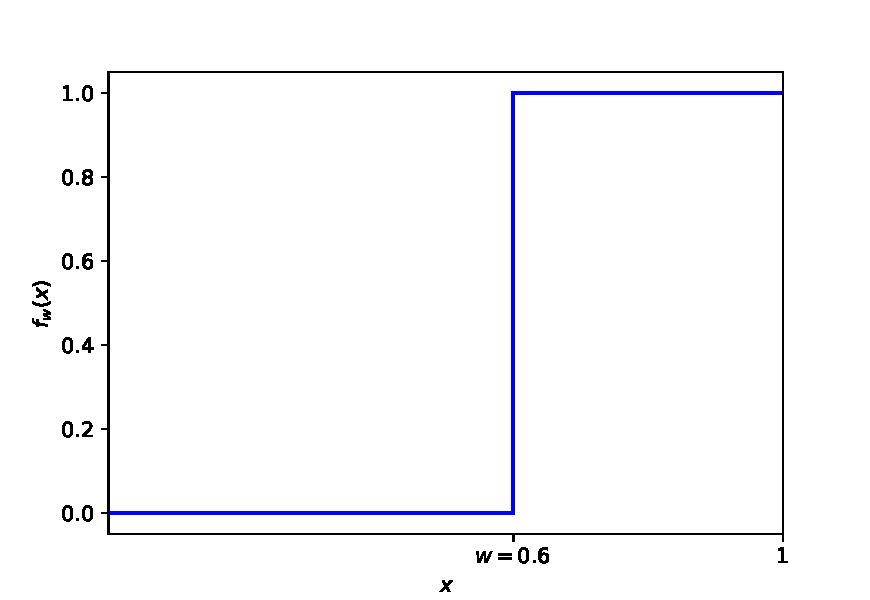
\includegraphics[width=12cm, height=6cm]{figures/threshold_fn.pdf}
%      \caption{An example of a linear threshold function $f_w(x) = \I(x \ge w)$ with $w = 0.6$.}
%     \label{fig:thresh-fn}
% \end{figure}

% \paragraph{Lower bracketing cover.}
% We first discretize the one-dimensional space of $w$'s at the scale of $\varepsilon$. Let $w_j = \set{\varepsilon, 2\varepsilon, \dots, N_{\varepsilon}\varepsilon}$, where $N_{\varepsilon} = \lceil \frac{1}{\varepsilon} \rceil$.

% The elements of the cover are given by $g_j = g_{w_j}\I( x \notin [w_j-\varepsilon, w_j])$. To check the first condition for a lower bracketing cover, notice that for any function $g_{w}$, outside $[w_j-\varepsilon, w_j]$ we have $g_w = g_{w_j}$  as $f_w = f_{w_j}$. Inside $[w_j-\varepsilon, w_j]$, we have $g_i = 0$ by definition. Therefore $g_i \le g_w$. To check the second condition for a lower bracketing cover, we follow the same argument as above and notice that the length of the interval $[w_j-\varepsilon, w_j]$ is $\varepsilon$ and the difference between $g_w$ and $g_j$ is bounded by 1, which gives $Pg_w \le Pg_i + \varepsilon$. We illustrate these conditions in \cref{fig:lb}.

% \begin{figure}
%     \centering
%     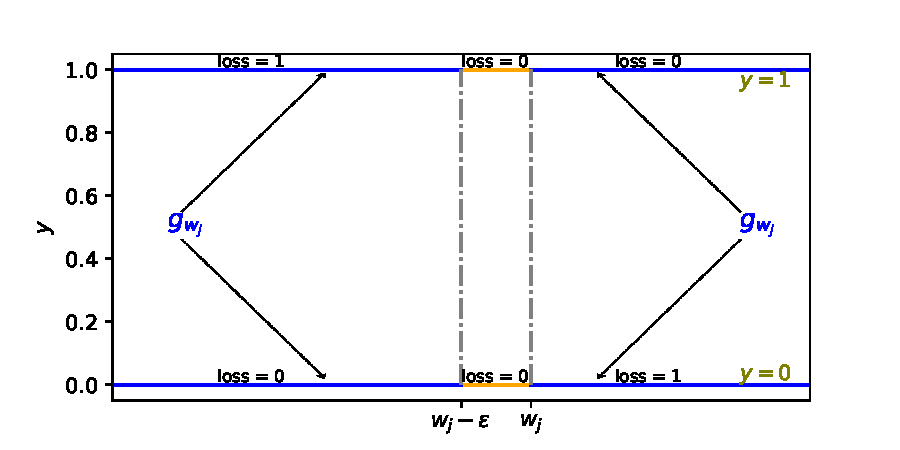
\includegraphics[width=12cm, height=6cm]{figures/loss.pdf}
%      \caption{Lower bracketing cover for linear threshold functions. The goal is to cover a function $g_w$ so that $w \in [w_j-\varepsilon, w_j]$. The cover element is $g_j = w_j \I(x \not in [w_j-\varepsilon, w_j])$. The indicated losses are for $g_j$ for the cases $y=0$ and $y=1$. The blue horizontal lines show the function. The blue horizontal lines indicate the intervals on which $g_j = g_{w_j}$ and the orange lines show the interval when $g_j = 0$.}
%     \label{fig:lb}
% \end{figure}

% We can also define general bracketing for two-sided uniform convergence.
% \begin{definition}[Bracketing]
%     Fix $\varepsilon > 0$. Let the function class $\cG$ be equipped with a pseudometric $d$ and let $g_i^L, g_i^U$ be functions from $cZ$ to $\R$ for $i \in [m]$. We call the set $\cG(\varepsilon) = \set{(g_1^L, g_1^U), \dots, (g_m^L, g_m^U) }$ an $\varepsilon$-bracket of $\cG$ under $d$ if $\forall g \in \cG$ there exists $j \in [m]$ such that (1) $g_j^L \le g \le g_j^U$; and (2) $d(g_j^L, g_j^U) \le \varepsilon$.
% \end{definition}
% % We remark that we lose some constant factors in the bounds while using bracketing.

% \section{Bounded Variance Condition}
% Multiplicative Chernoff gave fast convergence rates ($1/n$), however, it was restricted to the case when the predictors/losses are bounded and the loss is small. For some special cases when the variance of the loss is bounded, we can still get fast rates by exploiting the bounded variance property. This is given by Bernstein's inequality. But before delving into Bernstein's, let us define the bounded variance class and discuss some examples of loss classes that have bounded variance.   


% Let $\cZ = \cX \times \cY$ for some sets $\cX, \cY$ and $g:\cZ \to \cR$ be a measurable function. Further, let $P \in \cM_1(\cZ)$. The variance of $g$ measured against $P$ is given by $\Var_P(g) = P(g-Pg)^2$.

% \begin{definition}[Bounded variance class]
%     Fix $c_0, c_1 > 0$. Then the bounded variance class is defined as
%     \[
%         Var_{\cZ}(c_0, c_1, P) = \set{g: \cZ \to \R : \Var_P(g) \le c_0^2 + c_1Pg } \,.
%     \]
% \end{definition}

% \paragraph{Examples.}
% \begin{enumerate}
%     \item \textbf{Bounded functions.} If $0 \le g \le 1$, then $g \in \Var_{\cZ}(0, 1, P)$.

%     \item \textbf{Convex function class. }
%     For some set $\cX$, let $\cF \subset \cM(\cX,\R)$ and assume that $\cF$ is convex (i.e., for any $\alpha\in [0,1]$, $f,g\in \cF$, $\alpha f + (1-\alpha)g \in \cF$ also holds).
%     Let $\cZ = \cX \times \R$ and 
%     \[
%         \cG = \{ \ell_f \,:\, \ell_f: \cZ \to \R, \ell_f(x,y) = (f(x)-y)^2, f\in \cF \}\,.
%     \]
%     By abusing notation, we also write for this set  $\cG = \ell_{\text{sq}}\circ \cF$.
%     Let $P\in \cM_1(\cZ)$ be such that
%     for some $M>0$ constant, for any $g\in \cG$, $g(Z)\le M^2$ with probability one, where $Z\sim P$.
%     Define $g_* = \argmin_{g\in \cG} P g$ (which is assumed to exist) and 
%     \begin{align*}
%     \tilde\cG = \{ g - g_* \,:\, g\in \cG \}  \quad (= \cG - \{ g_*\})\,,
%     \end{align*}
%     so that $\inf_{\tilde{g} \in \tilde{\cG}} P\tilde{g} = 0$. Then, 
%     \begin{align*}
%     \tilde \cG \subset \Var_{\cZ}(0, 4M^2,P).
%     \end{align*}

%     \item \textbf{Best predictor not in the function class. }
%     Fix $M>0$. Let $\cF \subset \cM(\cX,[0,M])$ be set set of functions bounded in the interval $[0,M]$, $\cZ = \cX \times [0,M]$, $P\in \cM_1(\cZ)$ be a probability distribution over $\cZ$.
    
%     Now let $\cG = \ell_{\text{sq}} \circ \cF$ and $f_*(x) = \EE{Y|X=x}$ for $x\in \cX$ be the best predictor which may not be in the $\cF$. Define
%     \[
%         \tilde \cG = \cG - \{ \ell_{f_*} \}\,.
%     \]
%     Then,
%     \[
%         \tilde \cG \subset \Var_{\cZ}(0, 2M^2,P) \,.
%     \]  
% \end{enumerate}

 
\end{document}
